\documentclass[]{article}
\usepackage{lmodern}
\usepackage{amssymb,amsmath}
\usepackage{ifxetex,ifluatex}
\usepackage{fixltx2e} % provides \textsubscript
\ifnum 0\ifxetex 1\fi\ifluatex 1\fi=0 % if pdftex
  \usepackage[T1]{fontenc}
  \usepackage[utf8]{inputenc}
\else % if luatex or xelatex
  \ifxetex
    \usepackage{mathspec}
  \else
    \usepackage{fontspec}
  \fi
  \defaultfontfeatures{Ligatures=TeX,Scale=MatchLowercase}
\fi
% use upquote if available, for straight quotes in verbatim environments
\IfFileExists{upquote.sty}{\usepackage{upquote}}{}
% use microtype if available
\IfFileExists{microtype.sty}{%
\usepackage{microtype}
\UseMicrotypeSet[protrusion]{basicmath} % disable protrusion for tt fonts
}{}
\usepackage[margin=1in]{geometry}
\usepackage{hyperref}
\hypersetup{unicode=true,
            pdftitle={Music and Memory},
            pdfauthor={Lizhou Fan - lizhou@ucla.edu; Kaixin Wang - kaixinwang@ucla.edu; Huizi Yu - huiziy@ucla.edu},
            pdfborder={0 0 0},
            breaklinks=true}
\urlstyle{same}  % don't use monospace font for urls
\usepackage{longtable,booktabs}
\usepackage{graphicx,grffile}
\makeatletter
\def\maxwidth{\ifdim\Gin@nat@width>\linewidth\linewidth\else\Gin@nat@width\fi}
\def\maxheight{\ifdim\Gin@nat@height>\textheight\textheight\else\Gin@nat@height\fi}
\makeatother
% Scale images if necessary, so that they will not overflow the page
% margins by default, and it is still possible to overwrite the defaults
% using explicit options in \includegraphics[width, height, ...]{}
\setkeys{Gin}{width=\maxwidth,height=\maxheight,keepaspectratio}
\IfFileExists{parskip.sty}{%
\usepackage{parskip}
}{% else
\setlength{\parindent}{0pt}
\setlength{\parskip}{6pt plus 2pt minus 1pt}
}
\setlength{\emergencystretch}{3em}  % prevent overfull lines
\providecommand{\tightlist}{%
  \setlength{\itemsep}{0pt}\setlength{\parskip}{0pt}}
\setcounter{secnumdepth}{5}
% Redefines (sub)paragraphs to behave more like sections
\ifx\paragraph\undefined\else
\let\oldparagraph\paragraph
\renewcommand{\paragraph}[1]{\oldparagraph{#1}\mbox{}}
\fi
\ifx\subparagraph\undefined\else
\let\oldsubparagraph\subparagraph
\renewcommand{\subparagraph}[1]{\oldsubparagraph{#1}\mbox{}}
\fi

%%% Use protect on footnotes to avoid problems with footnotes in titles
\let\rmarkdownfootnote\footnote%
\def\footnote{\protect\rmarkdownfootnote}

%%% Change title format to be more compact
\usepackage{titling}

% Create subtitle command for use in maketitle
\providecommand{\subtitle}[1]{
  \posttitle{
    \begin{center}\large#1\end{center}
    }
}

\setlength{\droptitle}{-2em}

  \title{Music and Memory}
    \pretitle{\vspace{\droptitle}\centering\huge}
  \posttitle{\par}
  \subtitle{The Island Research Project}
  \author{Lizhou Fan - \href{mailto:lizhou@ucla.edu}{\nolinkurl{lizhou@ucla.edu}} \\ Kaixin Wang -
\href{mailto:kaixinwang@ucla.edu}{\nolinkurl{kaixinwang@ucla.edu}} \\ Huizi Yu - \href{mailto:huiziy@ucla.edu}{\nolinkurl{huiziy@ucla.edu}}}
    \preauthor{\centering\large\emph}
  \postauthor{\par}
      \predate{\centering\large\emph}
  \postdate{\par}
    \date{Statistics 101B - Spring 2019}

\usepackage{float} \floatplacement{figure}{H} \usepackage{lscape}
\usepackage{setspace} \setstretch{1.5}

\begin{document}
\maketitle

\begin{singlespace}
\tableofcontents
\end{singlespace}\newpage

\section{Abstract}\label{abstract}

The United States has experienced considerable growth in its elder
population in recent years. The number of older people is projected to
increase by 135\% between 2000 and 2050, and the population of people
aged 85 and over is projected to increase by 350\%. An ever growing
aging population will pose strains on work force as well as existing
health care. One common complication with aging is cognitive function
loss, and studies have demonstrated an interest in battling such loss
with non-medical treatments such as music. Thus, our study aims to
determine whether listening to music (more specifically which type of
music) have an effect on the performance of memory test for elders. We
chose Latin Square in order to control for the variability in
participants and the time memory test took place. We chose 25 male
islanders, from \texttt{The\ Island}\footnote{\href{http://island.maths.uq.edu.au}{\texttt{The\ Island:\ http://island.maths.uq.edu.au}}},
aged 65 to 89 from the town Macondo to perform 5x5 Latin Square 5 times
(each Latin Square contained 5 participants). Regarding the data
gathering process, we first administer the ``Memory Test Card'' task,
wait 5 minutes, then adminster the treatment (listening to 4 types of
music or no music), wait 10 minutes for treatment to take effect, and
then conduct the ``Memory Test Card'' again. The difference between two
``Memory Test Card'' scores are recorded. After data collection, we
first analyzed the box plots for each individual Latin Square, then we
created 6 ANOVA tables (5 for individual Latin Squares and 1 for the
combined model). The results showed that music is statistically
significant in 2 out of the 5 Latin Squares, but not significant in the
overall model. Further research topics are also discussed.

\section{Introduction}\label{introduction}

According to an annual report produced by the Administration for
Community Living, about one in every seven Americans is over the age of
65 in 2017, and the proportion will swell to one in five by 2040. Aging
is accompanied by declines in mental domains such as processing speed,
reasoning, memory and executive functions (Ian J. Deary, 2009). As
United States along with many other countries in the rest of world
enters an aging society, there is a growing interest in identifying
factors that can alleviate age-associated cognitive decline.

It has been suggested by some researches (Cirigliano, 2013; Michael,
David, Gerald \& Volker, 2014) that the temporal pattern structure in
music can enhance cognition and memory retention. This effect appears to
be especially significant for people with cognitive
deterioration/impairment. Such theory has been put to practice by
organizations such as \emph{MUSIC AND MEMORY}, a non-profit that brings
personalized music playlists to elders in nursing homes. They claim that
``Music is the most `fast-acting' non-drug approach to improving the
lives of all persons with dementia, Parkinson's, depression and other
behavioral challenges'' (2017 Impact Report, p.1).

Another interest of substantive researchers is the effect of different
genre of music on memory and cognition. There is a considerable amount
of publication dedicated to investigating the effect of Classical music
on performance and memory retention. Rausher, Shaw and Ky (1993) found
that listening to classical music improved intelligence and memory (the
``Mozart Effect'') and a British radio station specialised in western
classical music was shown to help listeners relax and improve brain
efficiency (Blanchard, 1979). Other studies compared different genres of
music and concluded fast-paced music such as Rap and Heavy Metal may
distract cognitive effects and lead to poorer performance (Dibben \&
Williamson, 2007; Smith \& Morris, 1977).

Due to music's accessibility as well as its universal presence, our
study is interested in testing whether there is theoretical support for
the uses of music as a means for memory improvement. We propose that
listening to music will lead to a statistically significant increase in
the memory test score. For this study, we apply four genres of music
(Country, Classical, Dance, Heavy Metal) as treatment variables and a
control variable (No Music). In this experiment, there are two goals.
First, we want to test if music is a valid treatment for increasing
memory performance; also, we want to find the best genre of music that
leads to said improvement.

\section{Methods}\label{methods}

\subsection{Participants}\label{participants}

We chose the virtual participants from the online resource the Island.
We found that female who age 65 or older are most susceptible to
cognitive impairment and are outperformed by men (in the same age group)
in fields of visuospatial, verbal processing, semantic and episodic
memory (Laws, K. R. 2016). Because memory retention differs in
individual (M. Karl Healey 2014), and in time of the day (A. D.
Baddeley, 2007), we use Latin Square to block by individual subject and
time of the day. In order to increase power as well as our error degrees
of freedom, we repeated this 5*5 Latin Square five times. This resulted
in our necessary sample size of 25 participants. Moreover, studies have
shown that cognitive impairment and dementia are are predicted to
increase proportionately more in developing regions, thus indicating a
potential association between the region of residence and cognitive
performance (WHO, 2013). We decide to hold this factor constant and
choose participants from the Town Macondo, where the population of
senior citizens is the largest. In order to obtain the 25 participants,
we went to the 64 neighbourhoods of Macondo and request consent from
female participants age 65 to 89.

\subsection{Design and Model}\label{design-and-model}

The Randomized Latin Square design is helpful when blocking two sources
of variation, person to person variability and order (time) of
treatment. Controlling these two factors, we would be more likely to
detect a significant result of the effect of our treatment, type of
music. Thus, we create a model accordingly:

\[y_{ijk} = \mu + \alpha_{i} + \beta_{j} + \gamma_{k} + \epsilon_{ijk},\ where\  i, j, k = 1, 2, 3, 4, 5\]

In the model, \(\alpha\) and \(\beta\) are the two blocking factors,
while \(\gamma\) represents the treatment. Moreover, we held-constant
three variables, including gender (male), region (the town of Macondo),
and age (between 65 and 89).

We created a 5x5 Latin Square matrix with each treatment occurring once
per row, and once per column. As the visualization below shows, these
music and non-music treatments were each assigned a letter from A to E,
i.e.~No music (A), Classical Music (B), Country Music (C), Dance Music
(D), and Heavy Metal Music (E).

\begin{figure}
\centering
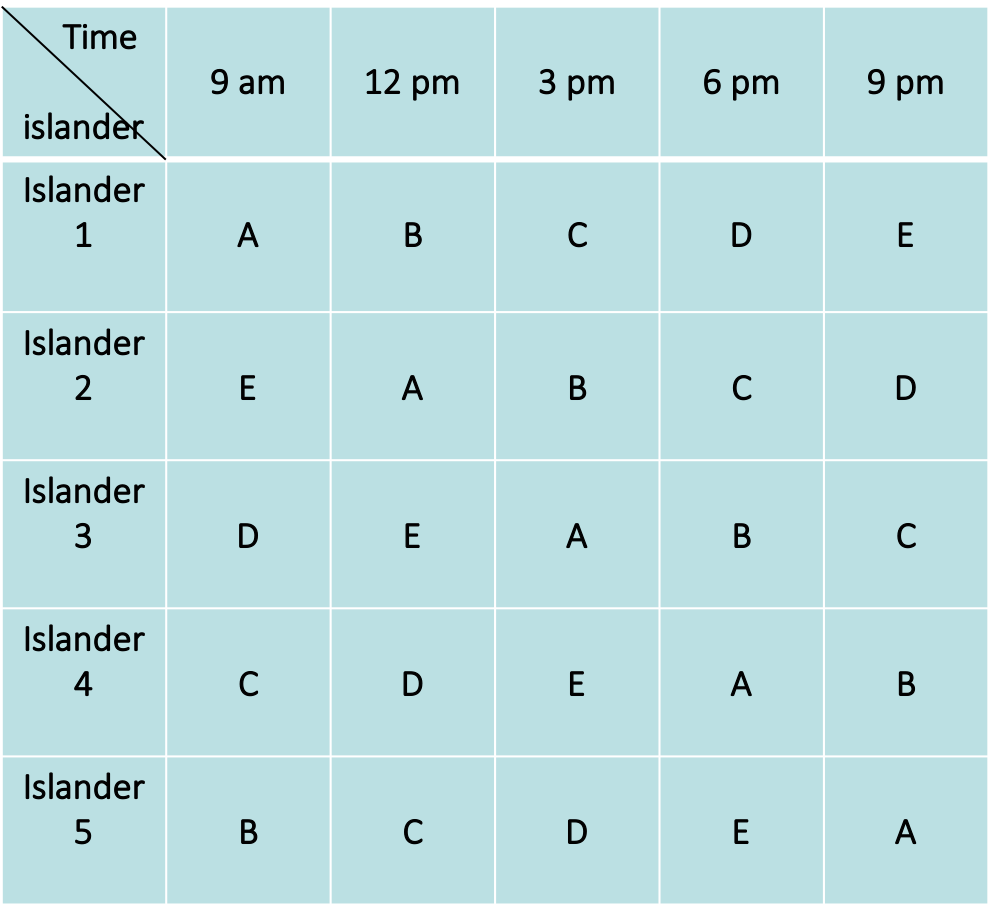
\includegraphics[width=0.45000\textwidth]{Square.png}
\caption{Latin Square Design}
\end{figure}

Then we created 5 replicates of the 5x5 Latin Square. To make a complete
random Latin-square design, we implemented the random assignment method
to shuffle the rows and columns. Using R, we assigned the numbers from 1
to 25 to the 25 participants and generated a random sequence (A) of
number from 1 to 25 (\texttt{set.seed(100000)}). Then we generated a
random sequence (B) of 1 to 5 (\texttt{set.seed(100000)}). We assigned
the participants indexed with the first five number of sequence A to the
Latin Square replicate indexed with the first number in sequence B and
the next five in A to the second number in B, etc. Finally, we randomly
permuted the columns, randomly permute the rows, and then assign the
treatments to the Latin letters in a random fashion. We ensured each
treatment occur once in each row and each column.

\subsection{Instrument}\label{instrument}

To conduct the study, we selected our participants from the Island to
gather our sample on the open platform The Island. To measure music's'
effects on memory of the simulated islanders on The Island, we used the
different genres of music under the ``Music'' task to assign treatment
at designated time and to record performance of ``Memory Test Card''.
Measurement errors were introduced and tolerated in the study as the
time of measurement cannot be exact (e.g., 9 am sharp), i.e.~we allowed
small measuring errors since it would not have significant impact on our
final result. As the data collection process of this project is highly
collocative, we used Google Sheet to record data collected on the
Island. For data analysis and data visualization, we used R and its
related packages and worded on the IDE of RStudio.

\subsection{Procedure}\label{procedure}

For each Latin Square, we first measured the performance of ``Memory
Test Card'', then waited for 5 minutes. Then, we assigned treatments
according to the randomized diagram; after the music treatment finishes,
we waited 10 minutes before performing the second ``Memory Test Card''.
We replicated this process for all 5 Latin Squares and recorded the
results into the Google Sheet.

\subsection{Data Analysis}\label{data-analysis}

Using R, we conducted an ANOVA test on the data. We first loaded the
data into R and used aov() function to analyze if there is any
difference among the effects of different genre of music on memory
retention among the 5 Latin Squares in the gathered data. In this
process, we obtained the degrees of freedom, sum of squares and mean sum
of squares for row and column blocks, the treatment, and their F and
p-values in the summary tables. Finally, we conducted a Tukey HSD
analysis to see how some certain variations by treatment predictor can
be explained. The result data structure is shown below.

\begin{longtable}[]{@{}llrrlr@{}}
\caption{Structure of data collected - Latin Square 1}\tabularnewline
\toprule
ID & treatment & before & after & time & difference\tabularnewline
\midrule
\endfirsthead
\toprule
ID & treatment & before & after & time & difference\tabularnewline
\midrule
\endhead
1 & A & 10 & 9 & 9:00 & -1\tabularnewline
1 & E & 10 & 8 & 12:00 & -2\tabularnewline
1 & B & 7 & 9 & 15:00 & 2\tabularnewline
1 & C & 9 & 9 & 18:00 & 0\tabularnewline
1 & D & 6 & 7 & 21:00 & 1\tabularnewline
\bottomrule
\end{longtable}

\section{Results}\label{results}

\subsection{Box Plots}\label{box-plots}

\textbf{Boxplot for each individual Latin Square:}

The median is represented by the black bar in the middle, where the
``box'' depicts the 1st and 3rd quantiles. Potential outliers are
displayed as black circles.

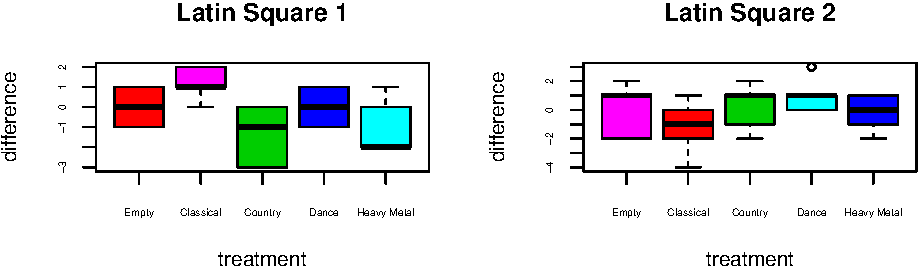
\includegraphics{STATS101B-Project-Code_files/figure-latex/unnamed-chunk-2-1.pdf}

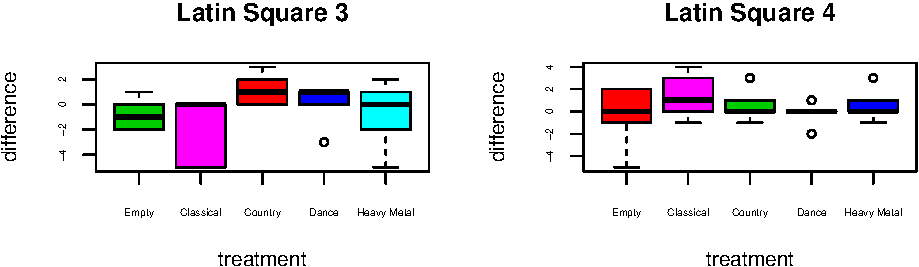
\includegraphics{STATS101B-Project-Code_files/figure-latex/unnamed-chunk-3-1.pdf}

\begin{figure}
\centering
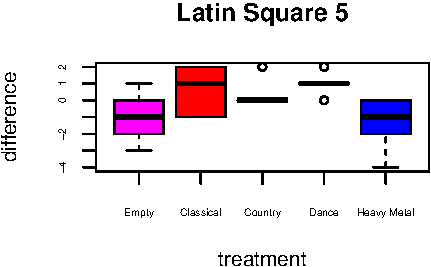
\includegraphics{STATS101B-Project-Code_files/figure-latex/unnamed-chunk-4-1.pdf}
\caption{Boxplots for individual Latin Squares}
\end{figure}

\textbf{Boxplot for all five Latin Squares combined:}

The median is represented by the black bar in the middle, where the
``box'' depicts the 1st and 3rd quantiles. Potential outliers are
displayed as black circles.

\begin{figure}
\centering
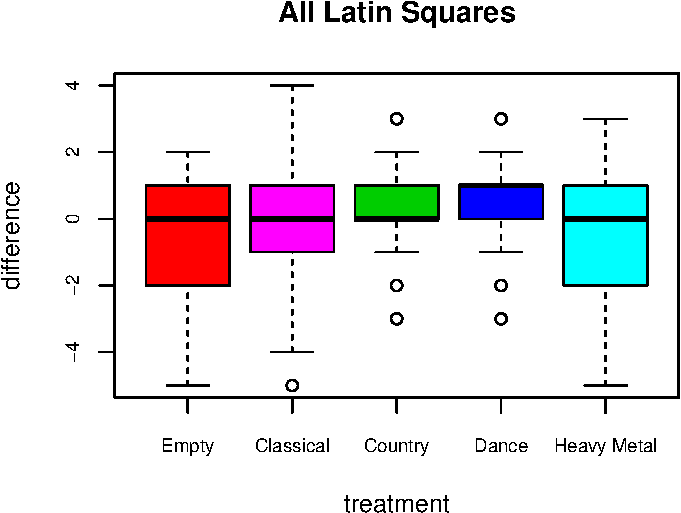
\includegraphics{STATS101B-Project-Code_files/figure-latex/unnamed-chunk-5-1.pdf}
\caption{Boxplot for all five Latin Squares}
\end{figure}

We began our exploratory data analysis by looking at the boxplots for
each Latin Square and the boxplot for all five Latin Squares combined.
We observe no significant difference in the mean of 5 music treatments
in Latin square 2, 3 and 4. In Latin square 1 and 5, there appears to be
a larger disparity between treatments. The boxplot for combined model
showed no significant difference in mean for each treatment either. We
proceed to ANOVA for further analysis.

\subsection{Analysis of Variance
(ANOVA)}\label{analysis-of-variance-anova}

We divided our analysis of variance (ANOVA) into two sections:

\textbf{Part 1: ANOVA of five individual Latin Squares:}

\textbf{Latin Square 1:}

\begin{longtable}[]{@{}cccccc@{}}
\caption{Analysis of Variance Table for Latin Square 1}\tabularnewline
\toprule
\begin{minipage}[b]{0.19\columnwidth}\centering\strut
~\strut
\end{minipage} & \begin{minipage}[b]{0.06\columnwidth}\centering\strut
Df\strut
\end{minipage} & \begin{minipage}[b]{0.10\columnwidth}\centering\strut
Sum Sq\strut
\end{minipage} & \begin{minipage}[b]{0.12\columnwidth}\centering\strut
Mean Sq\strut
\end{minipage} & \begin{minipage}[b]{0.12\columnwidth}\centering\strut
F value\strut
\end{minipage} & \begin{minipage}[b]{0.12\columnwidth}\centering\strut
Pr(\textgreater{}F)\strut
\end{minipage}\tabularnewline
\midrule
\endfirsthead
\toprule
\begin{minipage}[b]{0.19\columnwidth}\centering\strut
~\strut
\end{minipage} & \begin{minipage}[b]{0.06\columnwidth}\centering\strut
Df\strut
\end{minipage} & \begin{minipage}[b]{0.10\columnwidth}\centering\strut
Sum Sq\strut
\end{minipage} & \begin{minipage}[b]{0.12\columnwidth}\centering\strut
Mean Sq\strut
\end{minipage} & \begin{minipage}[b]{0.12\columnwidth}\centering\strut
F value\strut
\end{minipage} & \begin{minipage}[b]{0.12\columnwidth}\centering\strut
Pr(\textgreater{}F)\strut
\end{minipage}\tabularnewline
\midrule
\endhead
\begin{minipage}[t]{0.19\columnwidth}\centering\strut
\textbf{treatment}\strut
\end{minipage} & \begin{minipage}[t]{0.06\columnwidth}\centering\strut
4\strut
\end{minipage} & \begin{minipage}[t]{0.10\columnwidth}\centering\strut
20.56\strut
\end{minipage} & \begin{minipage}[t]{0.12\columnwidth}\centering\strut
5.14\strut
\end{minipage} & \begin{minipage}[t]{0.12\columnwidth}\centering\strut
8.965\strut
\end{minipage} & \begin{minipage}[t]{0.12\columnwidth}\centering\strut
0.001365\strut
\end{minipage}\tabularnewline
\begin{minipage}[t]{0.19\columnwidth}\centering\strut
\textbf{ID}\strut
\end{minipage} & \begin{minipage}[t]{0.06\columnwidth}\centering\strut
4\strut
\end{minipage} & \begin{minipage}[t]{0.10\columnwidth}\centering\strut
8.56\strut
\end{minipage} & \begin{minipage}[t]{0.12\columnwidth}\centering\strut
2.14\strut
\end{minipage} & \begin{minipage}[t]{0.12\columnwidth}\centering\strut
3.733\strut
\end{minipage} & \begin{minipage}[t]{0.12\columnwidth}\centering\strut
0.03387\strut
\end{minipage}\tabularnewline
\begin{minipage}[t]{0.19\columnwidth}\centering\strut
\textbf{time}\strut
\end{minipage} & \begin{minipage}[t]{0.06\columnwidth}\centering\strut
4\strut
\end{minipage} & \begin{minipage}[t]{0.10\columnwidth}\centering\strut
12.56\strut
\end{minipage} & \begin{minipage}[t]{0.12\columnwidth}\centering\strut
3.14\strut
\end{minipage} & \begin{minipage}[t]{0.12\columnwidth}\centering\strut
5.477\strut
\end{minipage} & \begin{minipage}[t]{0.12\columnwidth}\centering\strut
0.009582\strut
\end{minipage}\tabularnewline
\begin{minipage}[t]{0.19\columnwidth}\centering\strut
\textbf{Residuals}\strut
\end{minipage} & \begin{minipage}[t]{0.06\columnwidth}\centering\strut
12\strut
\end{minipage} & \begin{minipage}[t]{0.10\columnwidth}\centering\strut
6.88\strut
\end{minipage} & \begin{minipage}[t]{0.12\columnwidth}\centering\strut
0.5733\strut
\end{minipage} & \begin{minipage}[t]{0.12\columnwidth}\centering\strut
NA\strut
\end{minipage} & \begin{minipage}[t]{0.12\columnwidth}\centering\strut
NA\strut
\end{minipage}\tabularnewline
\bottomrule
\end{longtable}

\textbf{Latin Square 2:}

\begin{longtable}[]{@{}cccccc@{}}
\caption{Analysis of Variance Table for Latin Square 2}\tabularnewline
\toprule
\begin{minipage}[b]{0.19\columnwidth}\centering\strut
~\strut
\end{minipage} & \begin{minipage}[b]{0.06\columnwidth}\centering\strut
Df\strut
\end{minipage} & \begin{minipage}[b]{0.10\columnwidth}\centering\strut
Sum Sq\strut
\end{minipage} & \begin{minipage}[b]{0.12\columnwidth}\centering\strut
Mean Sq\strut
\end{minipage} & \begin{minipage}[b]{0.12\columnwidth}\centering\strut
F value\strut
\end{minipage} & \begin{minipage}[b]{0.12\columnwidth}\centering\strut
Pr(\textgreater{}F)\strut
\end{minipage}\tabularnewline
\midrule
\endfirsthead
\toprule
\begin{minipage}[b]{0.19\columnwidth}\centering\strut
~\strut
\end{minipage} & \begin{minipage}[b]{0.06\columnwidth}\centering\strut
Df\strut
\end{minipage} & \begin{minipage}[b]{0.10\columnwidth}\centering\strut
Sum Sq\strut
\end{minipage} & \begin{minipage}[b]{0.12\columnwidth}\centering\strut
Mean Sq\strut
\end{minipage} & \begin{minipage}[b]{0.12\columnwidth}\centering\strut
F value\strut
\end{minipage} & \begin{minipage}[b]{0.12\columnwidth}\centering\strut
Pr(\textgreater{}F)\strut
\end{minipage}\tabularnewline
\midrule
\endhead
\begin{minipage}[t]{0.19\columnwidth}\centering\strut
\textbf{treatment}\strut
\end{minipage} & \begin{minipage}[t]{0.06\columnwidth}\centering\strut
4\strut
\end{minipage} & \begin{minipage}[t]{0.10\columnwidth}\centering\strut
12.56\strut
\end{minipage} & \begin{minipage}[t]{0.12\columnwidth}\centering\strut
3.14\strut
\end{minipage} & \begin{minipage}[t]{0.12\columnwidth}\centering\strut
0.9691\strut
\end{minipage} & \begin{minipage}[t]{0.12\columnwidth}\centering\strut
0.4596\strut
\end{minipage}\tabularnewline
\begin{minipage}[t]{0.19\columnwidth}\centering\strut
\textbf{ID}\strut
\end{minipage} & \begin{minipage}[t]{0.06\columnwidth}\centering\strut
4\strut
\end{minipage} & \begin{minipage}[t]{0.10\columnwidth}\centering\strut
6.56\strut
\end{minipage} & \begin{minipage}[t]{0.12\columnwidth}\centering\strut
1.64\strut
\end{minipage} & \begin{minipage}[t]{0.12\columnwidth}\centering\strut
0.5062\strut
\end{minipage} & \begin{minipage}[t]{0.12\columnwidth}\centering\strut
0.7323\strut
\end{minipage}\tabularnewline
\begin{minipage}[t]{0.19\columnwidth}\centering\strut
\textbf{time}\strut
\end{minipage} & \begin{minipage}[t]{0.06\columnwidth}\centering\strut
4\strut
\end{minipage} & \begin{minipage}[t]{0.10\columnwidth}\centering\strut
6.96\strut
\end{minipage} & \begin{minipage}[t]{0.12\columnwidth}\centering\strut
1.74\strut
\end{minipage} & \begin{minipage}[t]{0.12\columnwidth}\centering\strut
0.537\strut
\end{minipage} & \begin{minipage}[t]{0.12\columnwidth}\centering\strut
0.7115\strut
\end{minipage}\tabularnewline
\begin{minipage}[t]{0.19\columnwidth}\centering\strut
\textbf{Residuals}\strut
\end{minipage} & \begin{minipage}[t]{0.06\columnwidth}\centering\strut
12\strut
\end{minipage} & \begin{minipage}[t]{0.10\columnwidth}\centering\strut
38.88\strut
\end{minipage} & \begin{minipage}[t]{0.12\columnwidth}\centering\strut
3.24\strut
\end{minipage} & \begin{minipage}[t]{0.12\columnwidth}\centering\strut
NA\strut
\end{minipage} & \begin{minipage}[t]{0.12\columnwidth}\centering\strut
NA\strut
\end{minipage}\tabularnewline
\bottomrule
\end{longtable}

\textbf{Latin Square 3:}

\begin{longtable}[]{@{}cccccc@{}}
\caption{Analysis of Variance Table for Latin Square 3}\tabularnewline
\toprule
\begin{minipage}[b]{0.19\columnwidth}\centering\strut
~\strut
\end{minipage} & \begin{minipage}[b]{0.06\columnwidth}\centering\strut
Df\strut
\end{minipage} & \begin{minipage}[b]{0.10\columnwidth}\centering\strut
Sum Sq\strut
\end{minipage} & \begin{minipage}[b]{0.12\columnwidth}\centering\strut
Mean Sq\strut
\end{minipage} & \begin{minipage}[b]{0.12\columnwidth}\centering\strut
F value\strut
\end{minipage} & \begin{minipage}[b]{0.12\columnwidth}\centering\strut
Pr(\textgreater{}F)\strut
\end{minipage}\tabularnewline
\midrule
\endfirsthead
\toprule
\begin{minipage}[b]{0.19\columnwidth}\centering\strut
~\strut
\end{minipage} & \begin{minipage}[b]{0.06\columnwidth}\centering\strut
Df\strut
\end{minipage} & \begin{minipage}[b]{0.10\columnwidth}\centering\strut
Sum Sq\strut
\end{minipage} & \begin{minipage}[b]{0.12\columnwidth}\centering\strut
Mean Sq\strut
\end{minipage} & \begin{minipage}[b]{0.12\columnwidth}\centering\strut
F value\strut
\end{minipage} & \begin{minipage}[b]{0.12\columnwidth}\centering\strut
Pr(\textgreater{}F)\strut
\end{minipage}\tabularnewline
\midrule
\endhead
\begin{minipage}[t]{0.19\columnwidth}\centering\strut
\textbf{treatment}\strut
\end{minipage} & \begin{minipage}[t]{0.06\columnwidth}\centering\strut
4\strut
\end{minipage} & \begin{minipage}[t]{0.10\columnwidth}\centering\strut
27.84\strut
\end{minipage} & \begin{minipage}[t]{0.12\columnwidth}\centering\strut
6.96\strut
\end{minipage} & \begin{minipage}[t]{0.12\columnwidth}\centering\strut
1.772\strut
\end{minipage} & \begin{minipage}[t]{0.12\columnwidth}\centering\strut
0.1992\strut
\end{minipage}\tabularnewline
\begin{minipage}[t]{0.19\columnwidth}\centering\strut
\textbf{ID}\strut
\end{minipage} & \begin{minipage}[t]{0.06\columnwidth}\centering\strut
4\strut
\end{minipage} & \begin{minipage}[t]{0.10\columnwidth}\centering\strut
29.04\strut
\end{minipage} & \begin{minipage}[t]{0.12\columnwidth}\centering\strut
7.26\strut
\end{minipage} & \begin{minipage}[t]{0.12\columnwidth}\centering\strut
1.849\strut
\end{minipage} & \begin{minipage}[t]{0.12\columnwidth}\centering\strut
0.1844\strut
\end{minipage}\tabularnewline
\begin{minipage}[t]{0.19\columnwidth}\centering\strut
\textbf{time}\strut
\end{minipage} & \begin{minipage}[t]{0.06\columnwidth}\centering\strut
4\strut
\end{minipage} & \begin{minipage}[t]{0.10\columnwidth}\centering\strut
10.24\strut
\end{minipage} & \begin{minipage}[t]{0.12\columnwidth}\centering\strut
2.56\strut
\end{minipage} & \begin{minipage}[t]{0.12\columnwidth}\centering\strut
0.652\strut
\end{minipage} & \begin{minipage}[t]{0.12\columnwidth}\centering\strut
0.6365\strut
\end{minipage}\tabularnewline
\begin{minipage}[t]{0.19\columnwidth}\centering\strut
\textbf{Residuals}\strut
\end{minipage} & \begin{minipage}[t]{0.06\columnwidth}\centering\strut
12\strut
\end{minipage} & \begin{minipage}[t]{0.10\columnwidth}\centering\strut
47.12\strut
\end{minipage} & \begin{minipage}[t]{0.12\columnwidth}\centering\strut
3.927\strut
\end{minipage} & \begin{minipage}[t]{0.12\columnwidth}\centering\strut
NA\strut
\end{minipage} & \begin{minipage}[t]{0.12\columnwidth}\centering\strut
NA\strut
\end{minipage}\tabularnewline
\bottomrule
\end{longtable}

\textbf{Latin Square 4:}

\begin{longtable}[]{@{}cccccc@{}}
\caption{Analysis of Variance Table for Latin Square 4}\tabularnewline
\toprule
\begin{minipage}[b]{0.19\columnwidth}\centering\strut
~\strut
\end{minipage} & \begin{minipage}[b]{0.06\columnwidth}\centering\strut
Df\strut
\end{minipage} & \begin{minipage}[b]{0.10\columnwidth}\centering\strut
Sum Sq\strut
\end{minipage} & \begin{minipage}[b]{0.12\columnwidth}\centering\strut
Mean Sq\strut
\end{minipage} & \begin{minipage}[b]{0.12\columnwidth}\centering\strut
F value\strut
\end{minipage} & \begin{minipage}[b]{0.12\columnwidth}\centering\strut
Pr(\textgreater{}F)\strut
\end{minipage}\tabularnewline
\midrule
\endfirsthead
\toprule
\begin{minipage}[b]{0.19\columnwidth}\centering\strut
~\strut
\end{minipage} & \begin{minipage}[b]{0.06\columnwidth}\centering\strut
Df\strut
\end{minipage} & \begin{minipage}[b]{0.10\columnwidth}\centering\strut
Sum Sq\strut
\end{minipage} & \begin{minipage}[b]{0.12\columnwidth}\centering\strut
Mean Sq\strut
\end{minipage} & \begin{minipage}[b]{0.12\columnwidth}\centering\strut
F value\strut
\end{minipage} & \begin{minipage}[b]{0.12\columnwidth}\centering\strut
Pr(\textgreater{}F)\strut
\end{minipage}\tabularnewline
\midrule
\endhead
\begin{minipage}[t]{0.19\columnwidth}\centering\strut
\textbf{treatment}\strut
\end{minipage} & \begin{minipage}[t]{0.06\columnwidth}\centering\strut
4\strut
\end{minipage} & \begin{minipage}[t]{0.10\columnwidth}\centering\strut
10.4\strut
\end{minipage} & \begin{minipage}[t]{0.12\columnwidth}\centering\strut
2.6\strut
\end{minipage} & \begin{minipage}[t]{0.12\columnwidth}\centering\strut
1.04\strut
\end{minipage} & \begin{minipage}[t]{0.12\columnwidth}\centering\strut
0.4266\strut
\end{minipage}\tabularnewline
\begin{minipage}[t]{0.19\columnwidth}\centering\strut
\textbf{ID}\strut
\end{minipage} & \begin{minipage}[t]{0.06\columnwidth}\centering\strut
4\strut
\end{minipage} & \begin{minipage}[t]{0.10\columnwidth}\centering\strut
10.4\strut
\end{minipage} & \begin{minipage}[t]{0.12\columnwidth}\centering\strut
2.6\strut
\end{minipage} & \begin{minipage}[t]{0.12\columnwidth}\centering\strut
1.04\strut
\end{minipage} & \begin{minipage}[t]{0.12\columnwidth}\centering\strut
0.4266\strut
\end{minipage}\tabularnewline
\begin{minipage}[t]{0.19\columnwidth}\centering\strut
\textbf{time}\strut
\end{minipage} & \begin{minipage}[t]{0.06\columnwidth}\centering\strut
4\strut
\end{minipage} & \begin{minipage}[t]{0.10\columnwidth}\centering\strut
33.2\strut
\end{minipage} & \begin{minipage}[t]{0.12\columnwidth}\centering\strut
8.3\strut
\end{minipage} & \begin{minipage}[t]{0.12\columnwidth}\centering\strut
3.32\strut
\end{minipage} & \begin{minipage}[t]{0.12\columnwidth}\centering\strut
0.0475\strut
\end{minipage}\tabularnewline
\begin{minipage}[t]{0.19\columnwidth}\centering\strut
\textbf{Residuals}\strut
\end{minipage} & \begin{minipage}[t]{0.06\columnwidth}\centering\strut
12\strut
\end{minipage} & \begin{minipage}[t]{0.10\columnwidth}\centering\strut
30\strut
\end{minipage} & \begin{minipage}[t]{0.12\columnwidth}\centering\strut
2.5\strut
\end{minipage} & \begin{minipage}[t]{0.12\columnwidth}\centering\strut
NA\strut
\end{minipage} & \begin{minipage}[t]{0.12\columnwidth}\centering\strut
NA\strut
\end{minipage}\tabularnewline
\bottomrule
\end{longtable}

\textbf{Latin Square 5:}

\begin{longtable}[]{@{}cccccc@{}}
\caption{Analysis of Variance Table for Latin Square 5}\tabularnewline
\toprule
\begin{minipage}[b]{0.19\columnwidth}\centering\strut
~\strut
\end{minipage} & \begin{minipage}[b]{0.06\columnwidth}\centering\strut
Df\strut
\end{minipage} & \begin{minipage}[b]{0.10\columnwidth}\centering\strut
Sum Sq\strut
\end{minipage} & \begin{minipage}[b]{0.12\columnwidth}\centering\strut
Mean Sq\strut
\end{minipage} & \begin{minipage}[b]{0.12\columnwidth}\centering\strut
F value\strut
\end{minipage} & \begin{minipage}[b]{0.12\columnwidth}\centering\strut
Pr(\textgreater{}F)\strut
\end{minipage}\tabularnewline
\midrule
\endfirsthead
\toprule
\begin{minipage}[b]{0.19\columnwidth}\centering\strut
~\strut
\end{minipage} & \begin{minipage}[b]{0.06\columnwidth}\centering\strut
Df\strut
\end{minipage} & \begin{minipage}[b]{0.10\columnwidth}\centering\strut
Sum Sq\strut
\end{minipage} & \begin{minipage}[b]{0.12\columnwidth}\centering\strut
Mean Sq\strut
\end{minipage} & \begin{minipage}[b]{0.12\columnwidth}\centering\strut
F value\strut
\end{minipage} & \begin{minipage}[b]{0.12\columnwidth}\centering\strut
Pr(\textgreater{}F)\strut
\end{minipage}\tabularnewline
\midrule
\endhead
\begin{minipage}[t]{0.19\columnwidth}\centering\strut
\textbf{treatment}\strut
\end{minipage} & \begin{minipage}[t]{0.06\columnwidth}\centering\strut
4\strut
\end{minipage} & \begin{minipage}[t]{0.10\columnwidth}\centering\strut
22.24\strut
\end{minipage} & \begin{minipage}[t]{0.12\columnwidth}\centering\strut
5.56\strut
\end{minipage} & \begin{minipage}[t]{0.12\columnwidth}\centering\strut
4.088\strut
\end{minipage} & \begin{minipage}[t]{0.12\columnwidth}\centering\strut
0.02564\strut
\end{minipage}\tabularnewline
\begin{minipage}[t]{0.19\columnwidth}\centering\strut
\textbf{ID}\strut
\end{minipage} & \begin{minipage}[t]{0.06\columnwidth}\centering\strut
4\strut
\end{minipage} & \begin{minipage}[t]{0.10\columnwidth}\centering\strut
5.84\strut
\end{minipage} & \begin{minipage}[t]{0.12\columnwidth}\centering\strut
1.46\strut
\end{minipage} & \begin{minipage}[t]{0.12\columnwidth}\centering\strut
1.074\strut
\end{minipage} & \begin{minipage}[t]{0.12\columnwidth}\centering\strut
0.4118\strut
\end{minipage}\tabularnewline
\begin{minipage}[t]{0.19\columnwidth}\centering\strut
\textbf{time}\strut
\end{minipage} & \begin{minipage}[t]{0.06\columnwidth}\centering\strut
4\strut
\end{minipage} & \begin{minipage}[t]{0.10\columnwidth}\centering\strut
13.44\strut
\end{minipage} & \begin{minipage}[t]{0.12\columnwidth}\centering\strut
3.36\strut
\end{minipage} & \begin{minipage}[t]{0.12\columnwidth}\centering\strut
2.471\strut
\end{minipage} & \begin{minipage}[t]{0.12\columnwidth}\centering\strut
0.1009\strut
\end{minipage}\tabularnewline
\begin{minipage}[t]{0.19\columnwidth}\centering\strut
\textbf{Residuals}\strut
\end{minipage} & \begin{minipage}[t]{0.06\columnwidth}\centering\strut
12\strut
\end{minipage} & \begin{minipage}[t]{0.10\columnwidth}\centering\strut
16.32\strut
\end{minipage} & \begin{minipage}[t]{0.12\columnwidth}\centering\strut
1.36\strut
\end{minipage} & \begin{minipage}[t]{0.12\columnwidth}\centering\strut
NA\strut
\end{minipage} & \begin{minipage}[t]{0.12\columnwidth}\centering\strut
NA\strut
\end{minipage}\tabularnewline
\bottomrule
\end{longtable}

\textbf{Part II: ANOVA for all five Latin Squares}:

\begin{longtable}[]{@{}cccccc@{}}
\caption{Analysis of Variance Table for five Latin
Squares}\tabularnewline
\toprule
\begin{minipage}[b]{0.19\columnwidth}\centering\strut
~\strut
\end{minipage} & \begin{minipage}[b]{0.06\columnwidth}\centering\strut
Df\strut
\end{minipage} & \begin{minipage}[b]{0.10\columnwidth}\centering\strut
Sum Sq\strut
\end{minipage} & \begin{minipage}[b]{0.12\columnwidth}\centering\strut
Mean Sq\strut
\end{minipage} & \begin{minipage}[b]{0.12\columnwidth}\centering\strut
F value\strut
\end{minipage} & \begin{minipage}[b]{0.12\columnwidth}\centering\strut
Pr(\textgreater{}F)\strut
\end{minipage}\tabularnewline
\midrule
\endfirsthead
\toprule
\begin{minipage}[b]{0.19\columnwidth}\centering\strut
~\strut
\end{minipage} & \begin{minipage}[b]{0.06\columnwidth}\centering\strut
Df\strut
\end{minipage} & \begin{minipage}[b]{0.10\columnwidth}\centering\strut
Sum Sq\strut
\end{minipage} & \begin{minipage}[b]{0.12\columnwidth}\centering\strut
Mean Sq\strut
\end{minipage} & \begin{minipage}[b]{0.12\columnwidth}\centering\strut
F value\strut
\end{minipage} & \begin{minipage}[b]{0.12\columnwidth}\centering\strut
Pr(\textgreater{}F)\strut
\end{minipage}\tabularnewline
\midrule
\endhead
\begin{minipage}[t]{0.19\columnwidth}\centering\strut
\textbf{treatment}\strut
\end{minipage} & \begin{minipage}[t]{0.06\columnwidth}\centering\strut
4\strut
\end{minipage} & \begin{minipage}[t]{0.10\columnwidth}\centering\strut
15.95\strut
\end{minipage} & \begin{minipage}[t]{0.12\columnwidth}\centering\strut
3.988\strut
\end{minipage} & \begin{minipage}[t]{0.12\columnwidth}\centering\strut
1.277\strut
\end{minipage} & \begin{minipage}[t]{0.12\columnwidth}\centering\strut
0.2849\strut
\end{minipage}\tabularnewline
\begin{minipage}[t]{0.19\columnwidth}\centering\strut
\textbf{ID}\strut
\end{minipage} & \begin{minipage}[t]{0.06\columnwidth}\centering\strut
24\strut
\end{minipage} & \begin{minipage}[t]{0.10\columnwidth}\centering\strut
70.83\strut
\end{minipage} & \begin{minipage}[t]{0.12\columnwidth}\centering\strut
2.951\strut
\end{minipage} & \begin{minipage}[t]{0.12\columnwidth}\centering\strut
0.9448\strut
\end{minipage} & \begin{minipage}[t]{0.12\columnwidth}\centering\strut
0.5436\strut
\end{minipage}\tabularnewline
\begin{minipage}[t]{0.19\columnwidth}\centering\strut
\textbf{time}\strut
\end{minipage} & \begin{minipage}[t]{0.06\columnwidth}\centering\strut
4\strut
\end{minipage} & \begin{minipage}[t]{0.10\columnwidth}\centering\strut
5.872\strut
\end{minipage} & \begin{minipage}[t]{0.12\columnwidth}\centering\strut
1.468\strut
\end{minipage} & \begin{minipage}[t]{0.12\columnwidth}\centering\strut
0.47\strut
\end{minipage} & \begin{minipage}[t]{0.12\columnwidth}\centering\strut
0.7576\strut
\end{minipage}\tabularnewline
\begin{minipage}[t]{0.19\columnwidth}\centering\strut
\textbf{Residuals}\strut
\end{minipage} & \begin{minipage}[t]{0.06\columnwidth}\centering\strut
92\strut
\end{minipage} & \begin{minipage}[t]{0.10\columnwidth}\centering\strut
287.4\strut
\end{minipage} & \begin{minipage}[t]{0.12\columnwidth}\centering\strut
3.124\strut
\end{minipage} & \begin{minipage}[t]{0.12\columnwidth}\centering\strut
NA\strut
\end{minipage} & \begin{minipage}[t]{0.12\columnwidth}\centering\strut
NA\strut
\end{minipage}\tabularnewline
\bottomrule
\end{longtable}

The ANOVA tables show that treatment is not significant in Latin Squares
2,3,4. The p-values are 0.45, 0.459, 0.199 and 0.426 respectively, which
are higher than the critical value of 0.05. Thus, we cannot conclude
that there is a relationship between Music treatment and change in
Memory Test performance. However, for Latin square 1 and 5, we can see
significant p-values for treatment: 0.0012 and 0.02564. Next, we combine
the five Latin Squares together to test the overall significance.
Unfortunately, treatment was not significant in the combined model
(p-value of 0.2849).

\subsection{Multiple groups
comparison}\label{multiple-groups-comparison}

\begin{figure}
\centering
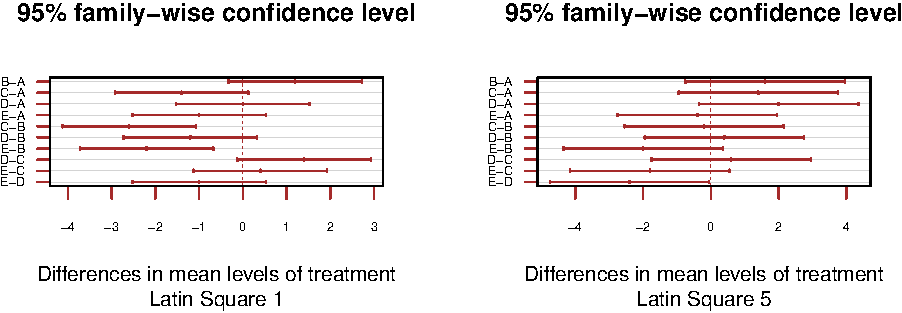
\includegraphics{STATS101B-Project-Code_files/figure-latex/unnamed-chunk-7-1.pdf}
\caption{Multiple groups comparison on Latin Square 1 and 5}
\end{figure}

Finding treatment significant in Latin square 1 and 5, we proceed to
conducting post-hoc TukeyHSD test to investigate which two music genres
lead to statistically different changes in memory performance. From the
plot for Latin Square 1, the two confidence intervals for pairwise
comparison for ``Country Music and Classical Music'', and for ``Heavy
Metal Music and Classical Music'' do not contain 0. This indicates that
for Latin square 1, the mean of Country Music and Classical Music are
statistically significant, as well as the mean of Heavy Metal Music and
Classical Music. However, in Latin square 5, all pairwise comparison
intervals contain 0. Thus, we conclude for Latin Square 5, none of the 5
treatment means are statistically different from each other.

\subsection{Residual Diagnostics}\label{residual-diagnostics}

\begin{figure}
\centering
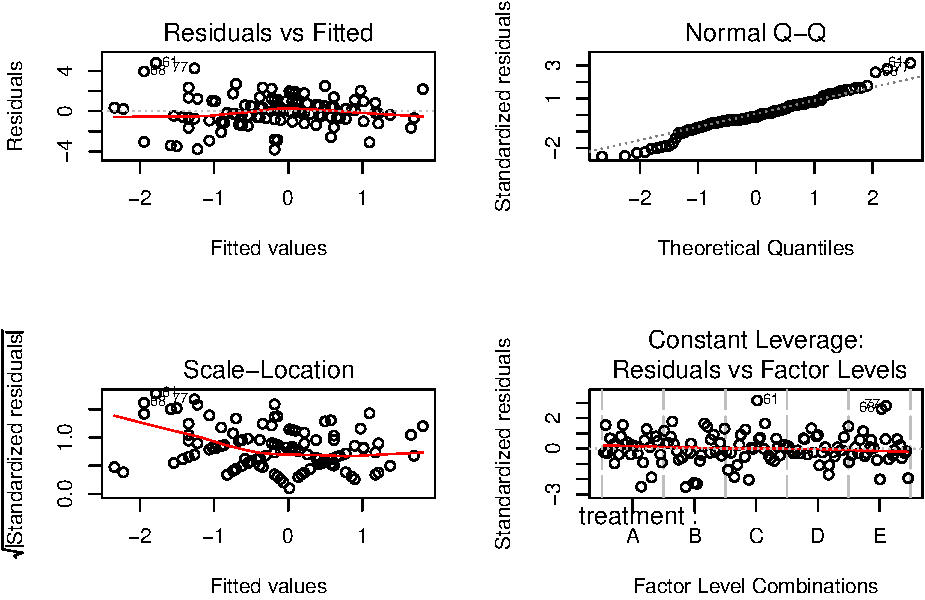
\includegraphics{STATS101B-Project-Code_files/figure-latex/unnamed-chunk-8-1.pdf}
\caption{Diagnostics plots for model difference \textasciitilde{}
treatment + ID + time}
\end{figure}

Based on the residuals vs.~fitted values plot, there is no certain
pattern in the graph, and the average value of error terms is mostly
around zero. This indicates that the assumption of independent error
terms with average value of zero is satisfied. Based on the normal
QQ-plot, we observe that most of the data points are around the
45-degree line through the origin. This indicates that the assumption of
normally distributed error terms is mostly satisfied. Based on the
\(\sqrt{standardized\ residuals}\) vs.~fitted values plot, we observe
that there is no obvious trend in the value of
\(\sqrt{standardized\ residuals}\). This indicates that the assumption
of constant variance of error terms is also mostly satisfied.

\section{Discussion}\label{discussion}

Using a complete random 5 times 5 Latin-square design with 5 replicates,
we collected data from 25 male islanders. After running our selected
tests on them, we did a bunch of analysis accordingly. We used box-plot
for exploration. Although there is no significant difference among the
mean of 5 music treatments in Latin square 2,3 and 4, In Latin square 1
and 5, there seems to exist a larger disparity between treatments.
Therefore, we further our study using ANOVA which demonstrated
significant results of Latin square 1 and 5 and confirmed our finding in
the explorative analysis.

The next step of our analysis, the multiple groups comparison, allowed
us to further investigate which two music genres lead to statistically
different changes in memory performance. As the line plots indicated,
both the mean of Country Music and Classical Music and the mean of Heavy
Metal Music and Classical Music are significantly effective on the
change of memory test performance. Also, after checking the assumptions
of our linear model of , we then conclude that our model,
\(y_{ijk} = \mu + \alpha_{i} + \beta_{j} + \gamma_{k} + \epsilon_{ijk},\ where\  i, j, k = 1, 2, 3, 4, 5\),
in which \(\alpha\) and \(\beta\) are the two blocking factors and
\(\gamma\) represents the treatment, is valid.

However, our results showed that there is limited evidence supporting
music's significance in affecting memory test score. This coincides with
the current controversial view on music's effectiveness in improving
memory. There are a few drawbacks in our design that might compromise
the results. The Latin Square design we employed does not assume
interaction between the rows, columns and the treatment factor. However,
it maybe possible that some individuals performed better in memory test
at specific time of the day. Moreover, although literature supported
that memory performance differs at different times of the day, it is not
a significant blocking factor in our model. As a result, choosing
another blocking factor may render treatment more significant. Another
potential aspect that may influence our result is the islanders' ability
to learn the Memory Test as the same test is repeated 5 times throughout
the day.

\section{Conclusion}\label{conclusion}

It is widely acknowledged that the memory problem, as one of the main
mental domain issues, is related to human aging and cognitive function
loss is a serious complication facing the aging US society. With a
shrinking workforce as the elders are unable to perform routine tasks,
the economy is likely suffer. Additional strains might be placed on the
health care system. Through our research, we aim at testing the
effectiveness of non-medical treatment, such as music of different
genre, as mediators to age related memory loss. Our results attempt to
support or refute the idea of using some certain genre of music as a
potential non-medical treatment for memory loss problems for senior
citizens.

To discuss the problem of our research and the possible further steps,
we visualized the the age distribution of 25 senior male islanders that
we sampled during the experiment. As the bar plot of the distribution
shows, two points are clear. For age distribution, most of the senior
male islanders have the age between 65 to 80 years old. Also, we
primarily focus on the investigation of male.

\begin{figure}
\centering
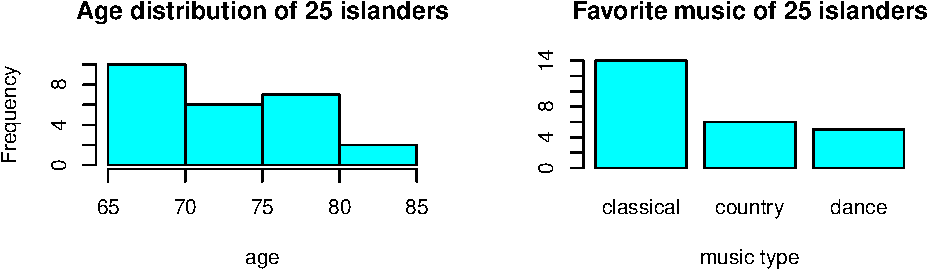
\includegraphics{STATS101B-Project-Code_files/figure-latex/unnamed-chunk-9-1.pdf}
\caption{Age distribution and results of the favorite music type survey}
\end{figure}

Since we are able to easily access the females on the island, we can
choose to sample female senior islanders in the experiment. In further
studies, we consider sample senior female islanders to investigate
whether music has effects on memory for them. It would also be helpful
to further investigate a larger range of age. It is important to notice
that, we accept individual variances, as the latin-square design can
handle them. To increase power, we would also like to repeat our
experiment with more Latin Squares and more samples.

After conducting the experiment on the Island, we also sent out a
post-experiment survey to the selected 25 islanders. The purpose of this
survey is to see which type of music is the islander's favorite, among
all four types of music (classical, country, dance and heavy metal
music). The result of the survey is shown as below. For their favorite
music types, most of the islanders sampled prefer listening to classical
music, while a small portion of the islanders prefer country and dance
music. One important observation is that none of the 25 islanders we
sampled prefer listening to heavy metal music, which may be closely
connected with results.

\newpage 

\section{References}\label{references}

\subsection{Journal References}\label{journal-references}

\begin{enumerate}
\def\labelenumi{(\arabic{enumi})}
\tightlist
\item
  \href{https://www.scientificamerican.com/article/music-and-the-brain-2006-09/}{\texttt{Music\ And\ The\ Brain}},
  Norman M. Weinberger. \emph{Scientific American}, September 1, 2006.
\item
  \href{https://med.stanford.edu/news/all-news/2007/07/music-moves-brain-to-pay-attention-stanford-study-finds.html}{\texttt{Music\ Moves\ Brain\ to\ Pay\ Attention}},
  Mitzi Baker. \emph{Stanford Medicine News Center}, August 1, 2007.
\item
  \href{https://www.cnn.com/2013/04/15/health/brain-music-research/index.html}{\texttt{This\ is\ Your\ Brain\ on\ Music}},
  Elizabeth Landau. \emph{CNN}, January 23, 2018.
\item
  \href{https://www.health.harvard.edu/staying-healthy/music-and-health}{\texttt{Music\ and\ health}},
  \emph{Harvard Medical School}, July 2011.
\item
  \href{https://www.encyclopedia.com/psychology/encyclopedias-almanacs-transcripts-and-maps/individual-differences-learning-and-memory}{\texttt{Individual\ Differences\ in\ Learning\ and\ Memory}}.
  \emph{Encyclopedia}, 2014.
\end{enumerate}

\subsection{Publication References}\label{publication-references}

\begin{enumerate}
\def\labelenumi{(\arabic{enumi})}
\tightlist
\item
  \href{https://search.proquest.com/docview/1701283142?pq-origsite=summon\&accountid=14512}{\texttt{A\ neuropsychological\ investigation\ of\ music,\ emotion,\ and\ autobiographical\ memory}},
  Belfi, Amy Meredith. \emph{University of Iowa}, 2015.
\item
  \href{https://search.proquest.com/docview/304910597?pq-origsite=summon\&accountid=14512}{\texttt{Music\ in\ the\ brain:\ Differences\ between\ musicians\ and\ non-musicians}},
  Orlando, Julie. \emph{University of Northern British Columbia
  (Canada)}, 2006.
\item
  \href{https://search.proquest.com/docview/2083960675?accountid=14512}{\texttt{Music\ for\ the\ Mind:\ A\ Study\ Into\ Musical\ Preferences,\ Personality\ Traits\ and\ Memory\ Retention}},
  Rogers, Rhiannon. \emph{Western Sydney University (Australia)}, 2018.
\item
  \href{https://search.proquest.com/docview/305228684?pq-origsite=summon\&accountid=14512}{\texttt{Music\ and\ cognitive\ abilities:\ A\ look\ at\ the\ Mozart\ Effect}},
  Bressler, Randy A. \emph{The Chicago School of Professional
  Psychology}, 2003.
\item
  \href{https://www.sciencedirect.com/science/article/pii/S1878875010001129}{\texttt{Music\ and\ the\ Brain}},
  Edward R. Laws, Jr. \emph{Harvard University}, 2010.
\item
  \href{https://scholar.utc.edu/cgi/viewcontent.cgi?article=1214\&context=mps}{\texttt{The\ effect\ of\ music\ genre\ on\ a\ memory\ task}},
  Bugter, Darragh \& Carden, Randy. \emph{Trevecca Nazarene University},
  2012.
\item
  \href{http://memory.psych.upenn.edu/files/pubs/HealEtal14.pdf}{\texttt{Individual\ Differences\ in\ Memory\ Search\ and\ Their\ Relation\ to\ Intelligence}},
  M. Karl Healey. \emph{University of Pennsylvania}, 2014.
\item
  \href{https://journals.sagepub.com/doi/10.1080/14640747008401939}{\texttt{Memory\ and\ time\ of\ day}},
  A. D. Baddeley, J. E. Hatter, Denise Scott \& Aileen Snashall.
  \emph{Quarterly Journal of Experimental Psychology}, 1970.
\item
  \href{https://scholar.utc.edu/mps/vol17/iss2/14}{\texttt{The\ effect\ of\ music\ genre\ on\ a\ memory\ task}},
  Bugter, Darragh and Carden, Randy. \emph{Modern Psychological Studies,
  Vol. 17, No.2, Article 14}, 2012.
\item
  \href{https://www.frontiersin.org/articles/10.3389/fnhum.2014.00395/full}{\texttt{Music\ mnemonics\ aid\ Verbal\ Memory\ and\ Induce\ Learning\ –\ Related\ Brain\ Plasticity\ in\ Multiple\ Sclerosis}},
  Thaut, Michael \& Peterson, David \& C McIntosh, Gerald \& Hömberg,
  Volker. \emph{Frontiers in human neuroscience}, 2014.
\item
  \href{https://journals.sagepub.com/doi/10.2466/pms.1998.86.3.835}{\texttt{Key\ Components\ of\ the\ Mozart\ Effect}},
  Frances H. Rauscher \& Gordon L. Shaw. \emph{University of Wiscomin,
  Osbkosb} \& \emph{University of California, Irvine}, 1998.
\end{enumerate}


\end{document}
